\section{Progettazione Logica}

\subsection{Modelli logici per il data mart}
Prendere gli schemi di fatto e tradurli in una implementazione coerenti con il modello scelto (ROLAP o MOLAP). Ci soffermeremo sul modello ROLAP. Esistono due tipi di schemi standard che si usano quando si implementa un cubo su una piattaforma ROLAP. Il principale è lo schema a stella ed è un modo classico per rappresentare un contenuto multidimensionale su un DB relazionale. Uno schema a stella è composto da:
\begin{itemize}
	\item 
	\textbf{Dimension Table}: una per ogni dimensione del cubo, in cui si ha una chiave primaria, che è un surrogato e dentro si hanno tutti gli attributi della gerarchia
	\item
	\textbf{Fact table}: importa al suo interno FK preso da tutte le DT. Tutte le FK insieme formano la chiave primaria e in più si trovano le misure
\end{itemize}

\textbf{Considerazioni}

Le DT sono completamente denormalizzate, non in terza forma normale e non si hanno problemi di sparsità in quanto vengono memorizzzate soltanto le tuple corrispondenti a punti dello spazio multidimensionale per cui esistono eventi. 
\begin{figure}[H]
	\centering
	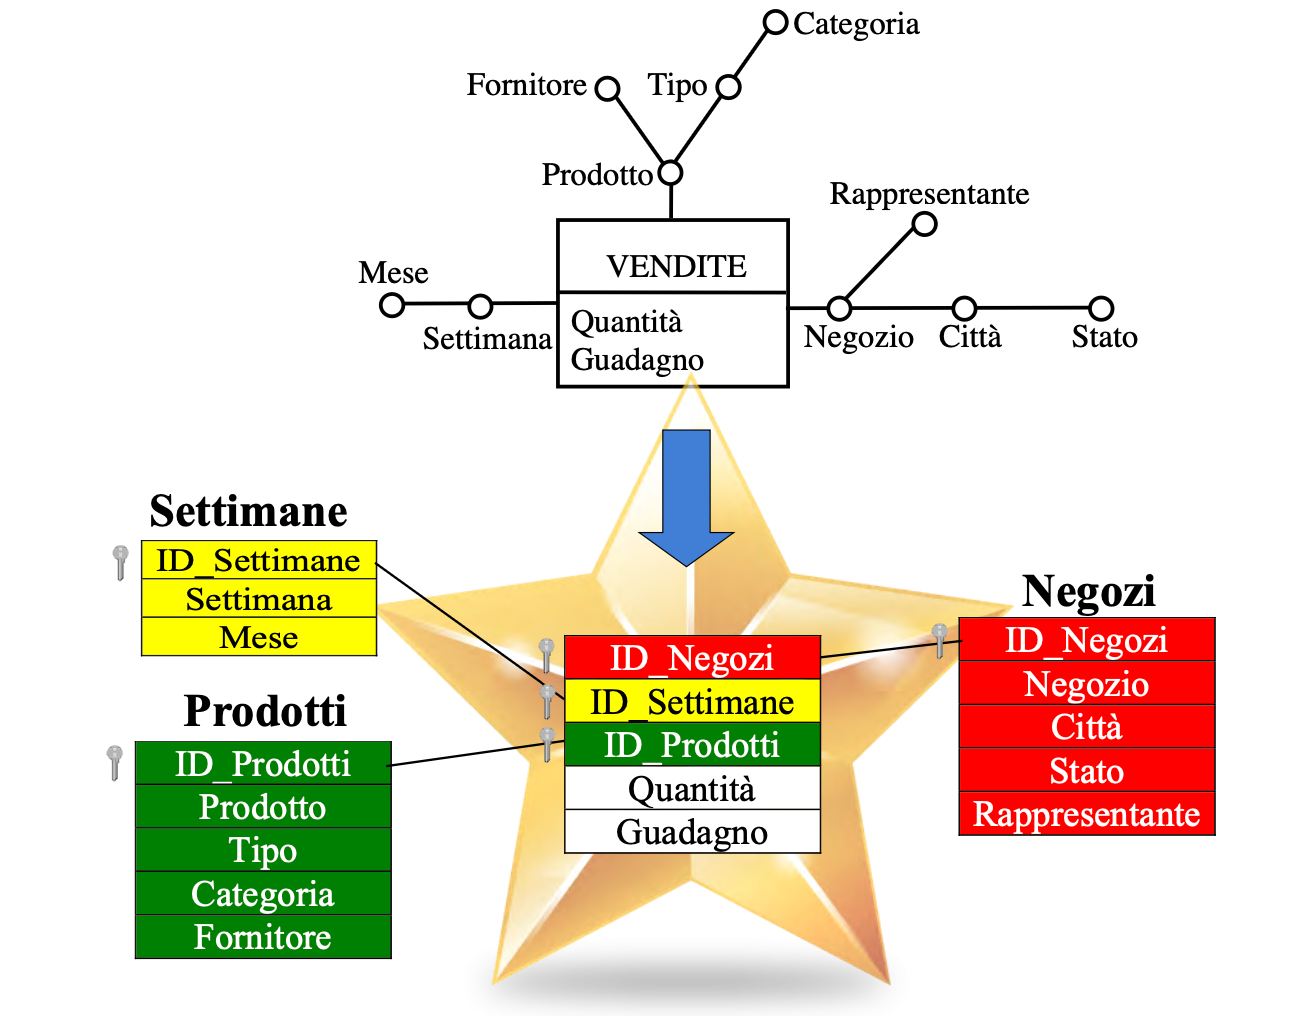
\includegraphics[width=0.6\linewidth]{img/stella}
	\caption{Schema a Stella}
	\label{fig:stella}
\end{figure}
Il secondo tipo di schema che si usa si chiama snowflake, il quale è una variante dello schema a stella, la cui caratteristica è che le DT vengono completamente o parzialmente normalizzate. 

\textbf{Considerazioni}

\begin{itemize}
	\item
	Lo spazio richiesto si riduce in linea di principio perché normalizzando elimino le ridondanze, ma è anche vero che ho aggiunto dei surrogati che nello schema a stella non si hanno
	\item 
	L’esecuzione di interrogazioni che coinvolgono solo gli attributi contenuti nella fact table e nelle dimension table primarie è avvantaggiata
	\item 
	Il tempo di esecuzione delle interrogazioni che coinvolgono attributi delle dimension table secondarie aumenta
\end{itemize}
\begin{figure}[H]
	\centering
	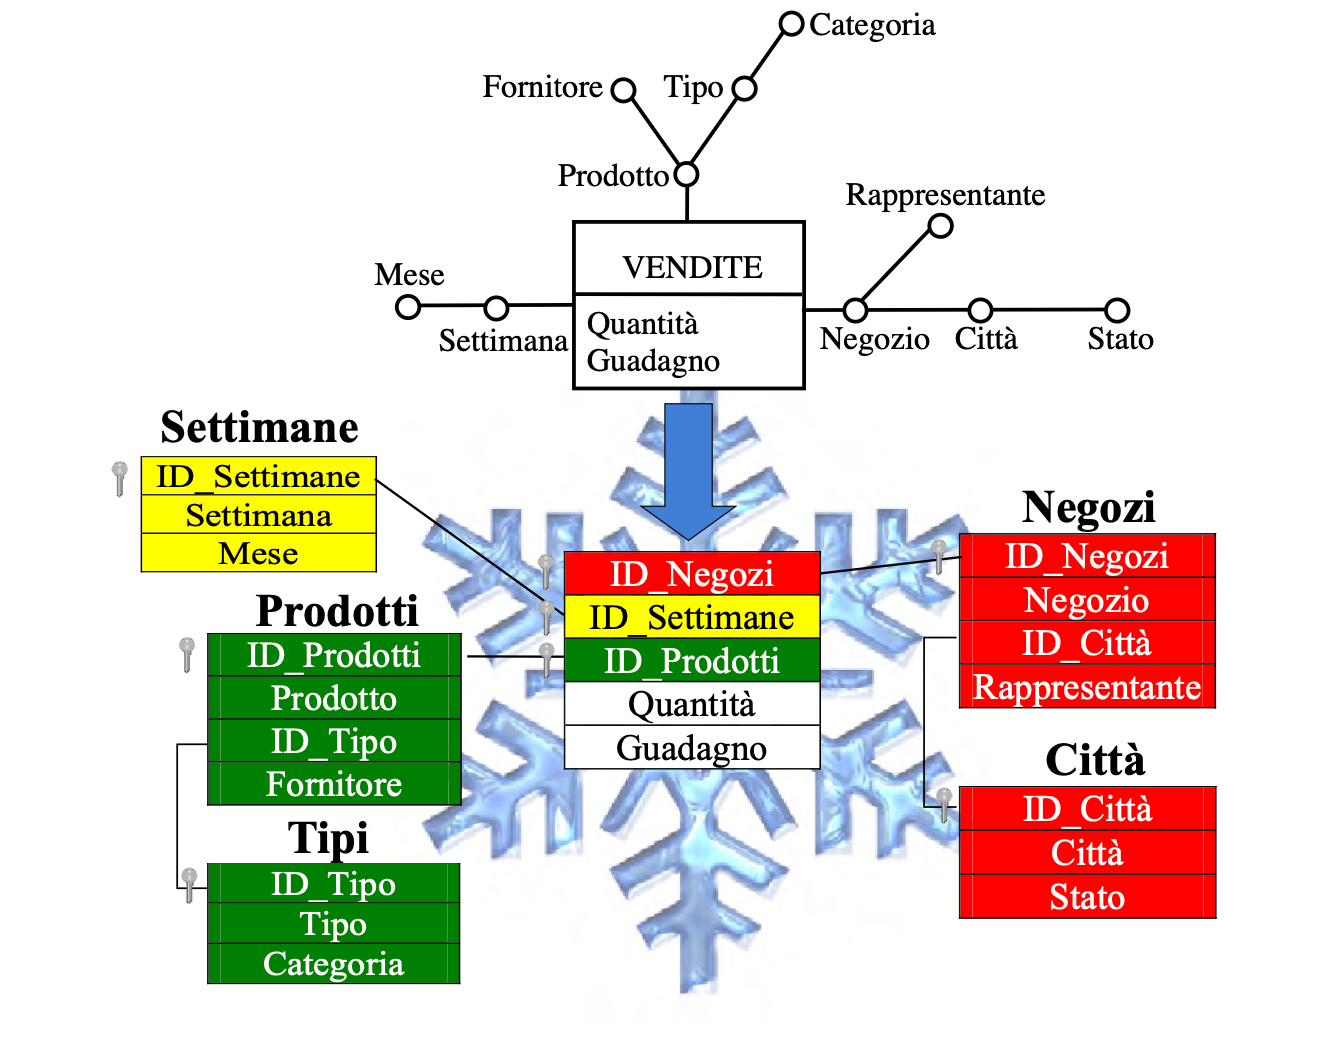
\includegraphics[width=0.6\linewidth]{img/snowflake}
	\caption{Snowflake}
	\label{fig:snowflake}
\end{figure}

\subsection{Le viste}

	

